% !TEX program = xelatex
% ============================================================================
%  POSN Computer Qualification — Quadratic Functions
%  Topic: ฟังก์ชันกำลังสอง (Quadratic Functions)
% ============================================================================

\documentclass[11pt, aspectratio=169]{beamer}
% ============================================================================
%  POSN Computer Qualification — Shared Beamer Preamble
%  Used by all topic slide decks. Compile with XeLaTeX.
% ============================================================================

% ---------- Thai language & font ----------
\usepackage{iftex}
\usepackage{fontspec}

% XeTeX-specific: enable Thai line breaking
\ifXeTeX
  \XeTeXlinebreaklocale{th}
\fi
% Noto Sans Thai — body text (clean modern sans-serif, handles all Thai)
\setmainfont{Noto Sans Thai}[
  UprightFont = Noto Sans Thai Light,
  BoldFont    = Noto Sans Thai Medium,
  Scale       = 0.9
]
\setsansfont{Noto Sans Thai}[
  UprightFont = Noto Sans Thai Light,
  BoldFont    = Noto Sans Thai Medium,
  Scale       = 0.9
]

% Noto Sans Thai — clean modern sans-serif for structural elements
\newfontfamily\headingfont{Noto Sans Thai}[
  UprightFont = Noto Sans Thai Medium,
  BoldFont    = Noto Sans Thai Bold,
  Scale       = 0.9
]

% --- Heading font for structural elements ---
\setbeamerfont{title}{family=\headingfont, series=\bfseries, size=\huge}
\setbeamerfont{subtitle}{family=\headingfont, series=\mdseries}
\setbeamerfont{author}{family=\headingfont, series=\mdseries}

% --- Custom Title Page ---
\defbeamertemplate{title page}{custom}[1][]{%
  \centering
  \vspace*{2cm}
  % Title — in white
  {\usebeamerfont{title}\color{white}\inserttitle\par}
  \vspace{0.6cm}
  % Subtitle — in white
  {\usebeamerfont{subtitle}\color{white}\insertsubtitle\par}
  \vspace{2.5cm}
  % Author — blue filled rounded box, white text
  \begin{center}
    \begin{tcolorbox}[arc=3mm, colback=boxBlue, colframe=boxBlue!80,
                      width=0.42\textwidth, halign=center,
                      left=1.5em, right=1.5em, top=0.8em, bottom=0.8em,
                      boxrule=1.5pt, coltext=white]
      \usebeamerfont{author}\insertauthor
    \end{tcolorbox}
  \end{center}
}
\setbeamertemplate{title page}[custom]
\setbeamerfont{frametitle}{family=\headingfont, series=\bfseries}
\setbeamerfont{section in toc}{family=\headingfont}
\setbeamerfont{page number in head/foot}{family=\headingfont}
\setbeamerfont{section title}{family=\headingfont, series=\bfseries}
\setbeamerfont{subsection title}{family=\headingfont}

% Monospace font (for code/verbatim)
\setmonofont{Latin Modern Mono}[Scale=0.9]

% ---------- Math ----------
\usepackage{amsmath, amssymb}

% ---------- Graphics ----------
\usepackage{graphicx}
\usepackage{tikz}

% ---------- String parsing (for section headers) ----------
\usepackage{xstring}

% ---------- Colored boxes ----------
\usepackage[skins, breakable, xparse]{tcolorbox}
% Note: we do NOT load the 'most' option — it predefines example/solution environments
% that would conflict with our custom boxes.

% --- Color definitions ---
\definecolor{boxBlue}{RGB}{41, 128, 185}
\definecolor{boxGreen}{RGB}{39, 174, 96}
\definecolor{boxOrange}{RGB}{230, 126, 34}
\definecolor{boxPurple}{RGB}{142, 68, 173}
\definecolor{boxBlueBg}{RGB}{235, 245, 255}
\definecolor{boxGreenBg}{RGB}{235, 255, 240}
\definecolor{boxOrangeBg}{RGB}{255, 245, 235}
\definecolor{boxPurpleBg}{RGB}{248, 240, 255}

% --- Explanation box (blue) — for definitions, concepts, notes ---
\newtcolorbox{explanation}[1][]{
  enhanced,
  breakable,
  arc         = 2mm,
  colback     = boxBlueBg,
  colframe    = boxBlue!50,
  title       = #1,
  fonttitle   = \bfseries\color{white},
  coltitle    = white,
  colbacktitle= boxBlue,
  attach boxed title to top left = {yshift=-2mm, xshift=2mm},
  boxed title style = {arc=2mm, size=small},
  before skip = 8pt,
  after skip  = 8pt
}

% --- Example box (green) — for worked examples ---
\newtcolorbox{exambox}[1][]{
  enhanced,
  breakable,
  arc         = 2mm,
  colback     = boxGreenBg,
  colframe    = boxGreen!50,
  title       = #1,
  fonttitle   = \bfseries\color{white},
  coltitle    = white,
  colbacktitle= boxGreen,
  attach boxed title to top left = {yshift=-2mm, xshift=2mm},
  boxed title style = {arc=2mm, size=small},
  before skip = 8pt,
  after skip  = 8pt
}

% --- Solution box (orange) — for solutions and answers ---
\newtcolorbox{solbox}[1][]{
  enhanced,
  breakable,
  arc         = 2mm,
  colback     = boxOrangeBg,
  colframe    = boxOrange!50,
  title       = #1,
  fonttitle   = \bfseries\color{white},
  coltitle    = white,
  colbacktitle= boxOrange,
  attach boxed title to top left = {yshift=-2mm, xshift=2mm},
  boxed title style = {arc=2mm, size=small},
  before skip = 8pt,
  after skip  = 8pt
}

% --- Intuition box (purple) — for plain-language explanations, analogies ---
\newtcolorbox{intuition}[1][]{
  enhanced,
  breakable,
  arc         = 2mm,
  colback     = boxPurpleBg,
  colframe    = boxPurple!50,
  title       = #1,
  fonttitle   = \bfseries\color{white},
  coltitle    = white,
  colbacktitle= boxPurple,
  attach boxed title to top left = {yshift=-2mm, xshift=2mm},
  boxed title style = {arc=2mm, size=small},
  before skip = 8pt,
  after skip  = 8pt
}

% ---------- Beamer theme ----------
\usetheme{Madrid}
\usecolortheme{default}

% --- Custom beamer colors (blue accent matching explanation boxes) ---
\setbeamercolor{structure}{fg=boxBlue}
\setbeamercolor{palette primary}{fg=white, bg=boxBlue}
\setbeamercolor{palette secondary}{fg=white, bg=boxBlue!80}
\setbeamercolor{palette tertiary}{fg=white, bg=boxBlue!60}
\setbeamercolor{block title}{fg=white, bg=boxBlue}
\setbeamercolor{block body}{fg=black, bg=boxBlueBg}

% Remove navigation symbols for clean look
\setbeamertemplate{navigation symbols}{}

% Note: Frame title prefix removed — \addtobeamertemplate conflicts with beamer internals

% --- Outline (Table of Contents) styling ---
\setbeamerfont{section in toc}{family=\headingfont, series=\mdseries}
\setbeamerfont{subsection in toc}{family=\headingfont, series=\mdseries}
\setbeamertemplate{section in toc}{%
  \leavevmode\leftskip=1.5em
  \textcolor{boxBlue}{\textbf{\large\inserttocsectionnumber.}}%
  \quad\inserttocsection\par
  \vspace{0.2em}
}
\setbeamertemplate{subsection in toc}{%
  \leavevmode\leftskip=4em
  \textcolor{boxBlue!60}{\small$\bullet$}%
  \quad\inserttocsubsection\par
  \vspace{0.1em}
}

% Section header slides — Thai in white, English in smaller light blue below
\AtBeginSection{
  \begin{frame}[plain]{}
    \vspace*{2cm}
    \begin{beamercolorbox}[sep=12pt, center, rounded=true, shadow=true]{palette primary}
      \IfSubStr{\secname}{(}{%
        \StrBefore{\secname}{(}[\sectionthai]%
        \StrBetween[1,1]{\secname}{(}{)}[\sectioneng]%
        \begin{tabular}{@{}c@{}}
          {\usebeamerfont{title}\sectionthai} \\[0.2em]
          {\usebeamerfont{subtitle}\color{boxBlue!60}\sectioneng}
        \end{tabular}%
      }{%
        {\usebeamerfont{title}\secname\par}%
      }
    \end{beamercolorbox}
    \vfill
  \end{frame}
}

% Subsection header slides — smaller, centered
\AtBeginSubsection{
  \begin{frame}[plain]{}
    \vfill
    \centering
    {\usebeamerfont{section title}\insertsubsectionhead\par}
    \vfill
  \end{frame}
}

% Minimal footer: page number only, right-aligned
\setbeamertemplate{footline}{
  \hfill\usebeamerfont{page number in head/foot}\insertframenumber{} / \inserttotalframenumber\hspace*{1em}\vspace*{0.5ex}
}

% ---------- Spacing & readability ----------
\linespread{1.2}

% ---------- Useful commands ----------

% Highlight important text in blue
\newcommand{\highlight}[1]{\textcolor{boxBlue}{\textbf{#1}}}

% Math set notation helpers
\newcommand{\R}{\mathbb{R}}
\newcommand{\N}{\mathbb{N}}
\newcommand{\Z}{\mathbb{Z}}
\newcommand{\Q}{\mathbb{Q}}

% ============================================================================
%  End of preamble
% ============================================================================


\title[ฟังก์ชันกำลังสอง]{ฟังก์ชันกำลังสอง}
\subtitle{Quadratic Functions — กราฟพาราโบลา, จุดยอด, ราก, การจัดรูป}
\author[None W. (Yuan)]{None W. (Yuan)}
\date{}

\begin{document}

\begin{frame}[plain]\titlepage\end{frame}
\begin{frame}{สารบัญ (Outline)}\tableofcontents\end{frame}

\begin{frame}{ก่อนเรียน (Prerequisites)}
  \begin{explanation}[สิ่งที่ควรรู้ก่อนเรียน]
    \begin{itemize}
      \item \textbf{ฟังก์ชัน} — นิยาม, โดเมน, เรนจ์, การหาค่าฟังก์ชัน
      \item \textbf{พหุนาม} — การแยกตัวประกอบ, กำลังสองสมบูรณ์
      \item \textbf{สมการ} — การแก้สมการกำลังสอง
    \end{itemize}
  \end{explanation}

  \begin{intuition}[ฟังก์ชันกำลังสองคืออะไร?]
    ฟังก์ชันที่มี $x^2$ เป็นพจน์ดีกรีสูงสุด — กราฟเป็นเส้นโค้งรูปตัว U หงายหรือคว่ำ
    เรียกว่า \textbf{พาราโบลา}
  \end{intuition}
\end{frame}

% ===========================================================================
%  SECTION 1: รูปแบบของฟังก์ชันกำลังสอง
% ===========================================================================
\section{รูปแบบของฟังก์ชันกำลังสอง}

\begin{frame}{ฟังก์ชันกำลังสอง: รูปแบบทั่วไป}
  \begin{explanation}[นิยาม]
    \textbf{ฟังก์ชันกำลังสอง} คือ $f(x) = ax^2 + bx + c$ โดย $a \neq 0$
  \end{explanation}

  \begin{columns}[T]
    \column{0.5\textwidth}
      \begin{explanation}[รูปร่างของกราฟ]
        \begin{itemize}
          \item $a > 0$: พาราโบลา \highlight{หงาย} $\cup$
          \item $a < 0$: พาราโบลา \highlight{คว่ำ} $\cap$
          \item $|a|$ มาก: กราฟแคบ
          \item $|a|$ น้อย: กราฟกว้าง
        \end{itemize}
      \end{explanation}
    \column{0.5\textwidth}
      \centering
      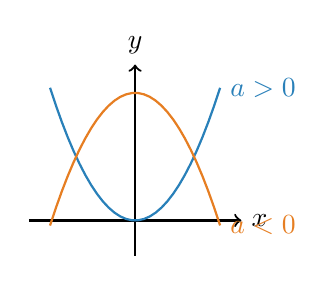
\begin{tikzpicture}[scale=0.9]
        \draw[->,thick] (-1.5,0) -- (1.5,0) node[right] {$x$};
        \draw[->,thick] (0,-0.5) -- (0,2.2) node[above] {$y$};
        % a > 0
        \draw[boxBlue, thick, domain=-1.2:1.2, samples=30]
          plot (\x, {1.3*\x*\x}) node[right] {$a>0$};
        % a < 0
        \draw[boxOrange, thick, domain=-1.2:1.2, samples=30]
          plot (\x, {-1.3*\x*\x + 1.8}) node[right] {$a<0$};
      \end{tikzpicture}
  \end{columns}
\end{frame}

\begin{frame}{สามรูปแบบของฟังก์ชันกำลังสอง}
  \begin{explanation}[1. รูปทั่วไป (Standard Form)]
    $f(x) = ax^2 + bx + c$

    เห็น \highlight{$y$-intercept} ทันที $= c$
  \end{explanation}

  \begin{explanation}[2. รูปจุดยอด (Vertex Form)]
    $f(x) = a(x - h)^2 + k$

    เห็น \highlight{จุดยอด} ทันที $= (h, k)$
  \end{explanation}

  \begin{explanation}[3. รูปผลคูณ (Factored Form)]
    $f(x) = a(x - r_1)(x - r_2)$

    เห็น \highlight{$x$-intercept (ราก)} ทันที: $x = r_1, r_2$
  \end{explanation}
\end{frame}

% ===========================================================================
%  SECTION 2: การจัดรูปกำลังสองสมบูรณ์
% ===========================================================================
\section{การจัดรูปกำลังสองสมบูรณ์ (Completing the Square)}

\begin{frame}{การเปลี่ยนรูปทั่วไปเป็นรูปจุดยอด}
  \begin{explanation}[วิธี: Completing the Square]
    $f(x) = ax^2 + bx + c \;\longrightarrow\; f(x) = a(x-h)^2 + k$

    โดย $h = -\frac{b}{2a}$ และ $k = f(h) = c - \frac{b^2}{4a}$
  \end{explanation}

  \begin{exambox}[ตัวอย่าง]
    $f(x) = x^2 - 6x + 5$
    $f(x) = (x^2 - 6x) + 5$ \quad
    บวกและลบ $(\frac{6}{2})^2 = 9$:

    $f(x) = (x^2 - 6x + 9) - 9 + 5 = (x-3)^2 - 4$

    \highlight{จุดยอด = $(3, -4)$, $a=1 > 0$ (หงาย)}
  \end{exambox}
\end{frame}

\begin{frame}{ตัวอย่าง: การจัดรูปกำลังสองสมบูรณ์ (ต่อ)}
  \begin{exambox}[ตัวอย่าง]
    \textbf{1.} $f(x) = 2x^2 + 8x + 3$:

    $2(x^2+4x)+3 = 2(x^2+4x+4)-8+3 = 2(x+2)^2-5$ \quad จุดยอด $(-2,-5)$

    \textbf{2.} $f(x) = -x^2 + 6x - 4$:

    $-(x^2-6x)-4 = -(x^2-6x+9)+9-4 = -(x-3)^2+5$ \quad จุดยอด $(3,5)$
  \end{exambox}
\end{frame}

% ===========================================================================
%  SECTION 3: จุดยอด แกนสมมาตร และค่าสูงสุด/ต่ำสุด
% ===========================================================================
\section{จุดยอด แกนสมมาตร และค่าสูงสุด/ต่ำสุด}

\begin{frame}{การหาจุดยอดและแกนสมมาตร}
  \begin{explanation}[สูตร]
    สำหรับ $f(x) = ax^2 + bx + c$:
    \begin{itemize}
      \item \textbf{แกนสมมาตร}: $x = h = -\frac{b}{2a}$
      \item \textbf{จุดยอด}: $\left(-\dfrac{b}{2a},\; f\!\left(-\dfrac{b}{2a}\right)\right)$
      \item \textbf{ค่าสูงสุด/ต่ำสุด}: $k = f(h)$
      \begin{itemize}
        \item $a > 0$: \highlight{ค่าต่ำสุด} $= k$ (หงาย)
        \item $a < 0$: \highlight{ค่าสูงสุด} $= k$ (คว่ำ)
      \end{itemize}
    \end{itemize}
  \end{explanation}

  \begin{exambox}
    $f(x) = 2x^2 - 8x + 5$

    $h = -\frac{-8}{2(2)} = \frac{8}{4} = 2$ \qquad $k = f(2) = 2(4) - 8(2) + 5 = 8 - 16 + 5 = -3$

    จุดยอด $= (2, -3)$, แกนสมมาตร $x = 2$, \highlight{ค่าต่ำสุด $= -3$}
  \end{exambox}
\end{frame}

% ===========================================================================
%  SECTION 4: รากของสมการกำลังสอง
% ===========================================================================
\section{รากของสมการกำลังสอง (Roots of Quadratic Equations)}

\begin{frame}{การหาราก (Discriminant \& Quadratic Formula)}
  \begin{explanation}[Discriminant]
    Discriminant: $\Delta = b^2 - 4ac$
    \begin{itemize}
      \item $\Delta > 0$: \highlight{2 รากจริง} (กราฟตัดแกน $x$ 2 จุด)
      \item $\Delta = 0$: \highlight{1 รากจริง} (กราฟสัมผัสแกน $x$)
      \item $\Delta < 0$: \highlight{ไม่มีรากจริง} (กราฟไม่ตัดแกน $x$)
    \end{itemize}
  \end{explanation}

  \begin{exambox}[สูตรและตัวอย่าง]
    $x = \dfrac{-b \pm \sqrt{b^2 - 4ac}}{2a}$

    $x^2 - 5x + 6 = 0$: \; $\Delta = 1$, \; $x = \frac{5 \pm 1}{2}$ \; $\rightarrow$ \; $x = 3, 2$
  \end{exambox}
\end{frame}

\begin{frame}{ผลบวกและผลคูณของราก}
  \begin{explanation}[สูตร (Vieta's Formulas)]
    สำหรับ $ax^2 + bx + c = 0$ ที่มีราก $r_1, r_2$: \\
    $r_1 + r_2 = -\frac{b}{a}$ \\
    $r_1 r_2 = \frac{c}{a}$ 
  \end{explanation}

  \begin{exambox}[ตัวอย่าง]
    $2x^2 - 6x + 4 = 0$ \quad $\rightarrow$ \quad $r_1 + r_2 = \frac{6}{2} = 3$,
    \; $r_1 r_2 = \frac{4}{2} = 2$

    ตรวจสอบ: รากคือ $x=1, x=2$ \quad $1+2=3$ $\checkmark$ \quad $1\times2=2$ $\checkmark$
  \end{exambox}

  \begin{intuition}
    \begin{itemize}
      \item หาผลบวก/ผลคูณโดยไม่ต้องแก้สมการ
      \item สร้างสมการกำลังสองจากรากที่กำหนด:
      $x^2 - (r_1+r_2)x + r_1r_2 = 0$
    \end{itemize}
  \end{intuition}
\end{frame}

\begin{frame}{ตัวอย่าง: สร้างสมการจากราก}
  \begin{exambox}[โจทย์ 1]
    จงสร้างสมการกำลังสองที่มีรากเป็น $3$ และ $-5$ โดยมี $a=1$
  \end{exambox}

  \begin{solbox}
    $r_1 + r_2 = 3 + (-5) = -2$, \quad $r_1 r_2 = 3(-5) = -15$

    $x^2 - (-2)x + (-15) = 0$

    $x^2 + 2x - 15 = 0$
  \end{solbox}

  \begin{exambox}[โจทย์ 2]
    กำหนด $r_1 + r_2 = 4$ และ $r_1 r_2 = 7$ จงหาค่าของ $r_1^2 + r_2^2$
  \end{exambox}

  \begin{solbox}
    $r_1^2 + r_2^2 = (r_1+r_2)^2 - 2r_1r_2 = 16 - 14 = 2$
  \end{solbox}
\end{frame}

% ===========================================================================
%  SECTION 5: อสมการกำลังสอง
% ===========================================================================
\section{อสมการกำลังสอง (Quadratic Inequalities)}

\begin{frame}{การแก้อสมการกำลังสอง}
  \begin{explanation}[วิธี]
    1. จัดรูปให้ข้างหนึ่งเป็น $0$ \quad
    2. หาราก \quad
    3. วิเคราะห์เครื่องหมายจากกราฟหรือ sign chart
  \end{explanation}

  \begin{exambox}[ตัวอย่าง]
    $x^2 - 4x + 3 \leq 0$: $(x-1)(x-3) \leq 0$, $a>0$ (หงาย)
    \highlight{$\rightarrow x \in [1, 3]$}

    $2x^2 - 3x - 2 > 0$: ราก $= 2, -\frac{1}{2}$, $a>0$ (หงาย)
    \highlight{$\rightarrow x \in (-\infty, -\frac{1}{2}) \cup (2, \infty)$}
  \end{exambox}
\end{frame}

% ===========================================================================
%  SECTION 6: การหาค่าสูงสุด/ต่ำสุดประยุกต์
% ===========================================================================
\section{โจทย์ประยุกต์}

\begin{frame}{โจทย์ปัญหาค่าสูงสุด/ต่ำสุด}
  \begin{exambox}[โจทย์]
    โยนวัตถุขึ้นไปในอากาศ ความสูง $h(t) = -5t^2 + 20t + 3$ เมตร ($t$ เป็นวินาที)
    จงหาความสูงสูงสุดและเวลาที่วัตถุถึงจุดสูงสุด
  \end{exambox}

  \begin{solbox}[วิธีทำ]
    $a = -5 < 0$ (คว่ำ) $\rightarrow$ มีค่าสูงสุดที่จุดยอด

    $t = -\frac{b}{2a} = -\frac{20}{2(-5)} = 2$ วินาที

    $h(2) = -5(4) + 20(2) + 3 = -20 + 40 + 3 = 23$ เมตร

    \highlight{สูงสุด $23$ เมตร ที่ $t = 2$ วินาที}
  \end{solbox}
\end{frame}

\begin{frame}{โจทย์ปัญหา: พื้นที่มากที่สุด}
  \begin{exambox}[โจทย์]
    ต้องการล้อมรั้วสี่เหลี่ยมผืนผ้าติดกำแพง (ด้านหนึ่งใช้กำแพง) ด้วยลวดหนามยาว 60 เมตร
    จงหาพื้นที่มากที่สุดที่เป็นไปได้
  \end{exambox}

  \begin{solbox}[วิธีทำ]
    ให้ด้านกว้าง $= x$, ด้านยาว $= 60 - 2x$ \quad (ใช้กำแพงแทนรั้ว 1 ด้าน)

    พื้นที่ $A(x) = x(60-2x) = -2x^2 + 60x$

    ค่าสูงสุดที่ $x = -\frac{60}{2(-2)} = 15$ ม.

    $A(15) = -2(225) + 60(15) = -450 + 900 = 450$ ตร.ม.

    \highlight{พื้นที่มากที่สุด $= 450$ ตร.ม.}
  \end{solbox}
\end{frame}

\begin{frame}{โจทย์ปัญหา: กำไรสูงสุด}
  \begin{exambox}[โจทย์]
    ร้านค้าแห่งหนึ่งขายสินค้าได้ $x$ ชิ้นต่อวัน โดยมีกำไรต่อวันเป็น
    $P(x) = -2x^2 + 120x - 500$ บาท
    จงหาจำนวนสินค้าที่ทำให้ได้กำไรสูงสุด และกำไรสูงสุดเป็นเท่าใด
  \end{exambox}

  \begin{solbox}[วิธีทำ]
    $P(x) = -2x^2 + 120x - 500$ \quad ($a = -2 < 0$ คว่ำ มีค่าสูงสุด)

    $x = -\dfrac{b}{2a} = -\dfrac{120}{2(-2)} = \dfrac{120}{4} = 30$ ชิ้น

    $P(30) = -2(900) + 120(30) - 500 = -1800 + 3600 - 500 = 1300$ บาท

    \highlight{ขายวันละ $30$ ชิ้น ได้กำไรสูงสุด $1{,}300$ บาท}
  \end{solbox}

  \begin{intuition}
    สมการกำไรมักอยู่ในรูป $P(x) = -ax^2 + bx - c$
    — จุดยอดคือจุดที่ได้กำไรสูงสุด
  \end{intuition}
\end{frame}

\begin{frame}{โจทย์ปัญหา: เงื่อนไขราก}
  \begin{exambox}[ตัวอย่าง]
    \textbf{1.} $x^2 + kx + 4 = 0$ มีหนึ่งรากเมื่อ $\Delta = 0$:

    $k^2 - 16 = 0$ \quad $\rightarrow$ \quad $k = \pm 4$

    \medskip
    \textbf{2.} $x^2 + mx + 9 = 0$ สัมผัสแกน $x$ เมื่อ $\Delta = 0$:

    $m^2 - 36 = 0$ \quad $\rightarrow$ \quad $m = \pm 6$
  \end{exambox}

  \begin{intuition}[สรุป]
    สัมผัสแกน $x$ $\iff$ $\Delta = 0$ $\iff$ มีหนึ่งราก (รากซ้ำ) $\iff$ จุดยอดอยู่บนแกน $x$
  \end{intuition}
\end{frame}

% ===========================================================================
%  SUMMARY
% ===========================================================================
\section{สรุป}

\begin{frame}{สรุปเนื้อหา}
  \begin{explanation}[สิ่งที่ได้เรียนรู้]
    \begin{columns}[T]
      \column{0.5\textwidth}
        \begin{itemize}
          \item \textbf{รูปแบบ}: ทั่วไป, จุดยอด, ผลคูณ
          \item \textbf{การจัดรูป}: $h = -\frac{b}{2a}$, $k = f(h)$
          \item \textbf{แกนสมมาตร}: $x = -\frac{b}{2a}$
          \item \textbf{ค่าสูงสุด/ต่ำสุด}: $a>0$ ต่ำสุด, $a<0$ สูงสุด
        \end{itemize}
      \column{0.5\textwidth}
        \begin{itemize}
          \item \textbf{Discriminant}: $\Delta = b^2-4ac$
          \item \textbf{สูตรกำลังสอง}: $x = \frac{-b \pm \sqrt{\Delta}}{2a}$
          \item \textbf{ผลบวก/ผลคูณ}: $r_1+r_2 = -b/a$, $r_1r_2 = c/a$
          \item \textbf{อสมการ}: แยกตัวประกอบ + sign chart
        \end{itemize}
    \end{columns}
  \end{explanation}
  \begin{center}
    \large เอกสารนี้เป็นส่วนหนึ่งของเนื้อหาเตรียมสอบ \textbf{สอวน. คอมพิวเตอร์}
  \end{center}
\end{frame}

\end{document}
